\documentclass[a4paper, 12pt]{article}

\newcommand\tab[1][.6cm]{\hspace*{#1}}
\usepackage[portuges]{babel}
\usepackage[utf8]{inputenc}
\usepackage{amsmath}
\usepackage{indentfirst}
\usepackage{graphicx}
\usepackage{multicol,lipsum}
\usepackage{blindtext}
\usepackage{verbatim}
\usepackage{textcomp}
\usepackage{hyperref}
\usepackage{float}
\usepackage{url}

\usepackage[most]{tcolorbox}

% Dirac's notation
\usepackage{mathtools}
\DeclarePairedDelimiter\bra{\langle}{\rvert}
\DeclarePairedDelimiter\ket{\lvert}{\rangle}
\DeclarePairedDelimiterX\braket[2]{\langle}{\rangle}{#1\,\delimsize\vert\,\mathopen{}#2}

\begin{document}
%\maketitle

\begin{titlepage}
	\begin{center}
	
	\begin{figure}[ht]
    \centering
    
\includegraphics[width=.44\textwidth]{Images/LogoUFSJ.PNG}
    \label{fig:Capturar.PNG}
    \end{figure}

    	\Huge{Universidade Federal São João del Rei}\\
		\Large{Curso de Ciência da Computação}\\ 

        \vspace{90pt}
        \textbf{\LARGE{
        \\
        \\
        \\
        Trabalho Prático I:\\
        Relatório\\
        \vspace{0.5cm}
        \Large{Computação Paralela}
        \\
        \\
        \\
        }}
        
		\title{{\large{Título}}}
		\vspace{1.5cm}
	\end{center}
	    
    \begin{flushleft}
		\begin{tabbing}
		\\
		\\
		\\	
		\large{Discente: Julio Cesar da Silva Rodrigues}\\
	    \\
		\large{Docente: Rafael Sachetto Oliveira}\\
	    \end{tabbing}
    \end{flushleft}
	\vspace{1cm}
	
	\begin{center}
		\vspace{\fill}
			Outubro\\
		    2023
	\end{center}
\end{titlepage}

\tableofcontents
\newpage
\section{Introdução}

Neste trabalho, é apresentada uma solução de paralelização em um problema de se encontrar a quantidade de divisores, dada uma entrada variável com quaisquer valores. O objetivo principal é identificar porções da implementação que por talvez apresentarem maior uso computacional, possam ser paralelizadas utilizando a biblioteca \textbf{OpenMPI}\footnotemark \hspace{0.1cm}com o paradigma de computação paralela mestre-escravo para obter ganhos significativos em tempo de execução.

\footnotetext[1]{\scriptsize{Mais informações disponíveis em: \url{https://www.open-mpi.org/}}}

Além disso, é realizada uma análise detalhada quanto a como cada tipo de entrada afeta no tempo de execução do programa, a granularidade (i.e., taxa entre computação e comunicação dos processos), uso de recursos computacionais (CPU, memória principal, ...) e o potencial \emph{speed up} que o aumento da paralelização (i.e., número de processos) proporciona.

\section{Desenvolvimento}

Toda a concepção do cálculo do número de divisores, assim como as funções responsáveis pela paralelização e manipulação de E/S foram implementadas na linguagem C (excetuando a análise gráfica de resultados e geração dos instâncias de teste, estes que foram gerados utilizando a linguagem Python\footnotemark \hspace{0.1cm}com auxílio das bibliotecas Matplotlib\footnotemark \hspace{0.1cm}e seaborn\footnotemark). A implementação foi desenvolvida com o auxílio da ferramenta de controle de versionamento GitHub\footnotemark, e encontra-se disponível publicamente no repositório \url{https://github.com/juliorodrigues07/parallel_primes}.

\footnotetext[2]{\scriptsize{Mais informações disponíveis em: \url{https://www.python.org/}}}
\footnotetext[3]{\scriptsize{Mais informações disponíveis em: \url{https://matplotlib.org/}}}
\footnotetext[4]{\scriptsize{Mais informações disponíveis em: \url{https://seaborn.pydata.org/}}}
\footnotetext[5]{\scriptsize{Mais informações disponíveis em: \url{https://github.com}}}

A organização do código se apresenta de forma bastante simples. Existem um par de arquivos de código fonte (juntamente com seus \emph{headers .h} associados) que são responsáveis por realizar as manipulações de entrada e saída (\emph{data\_management}) e calcular o número de divisores de cada valor da entrada (\emph{divisors}). No código fonte principal (\emph{main.c}) encontra-se a utilização da biblioteca OpenMPI para introdução do paralelismo ao programa. Além disso, também existe um segundo arquivo (\emph{sequential.c}) para execução sequencial para fins de comparação de resultados.

\subsection{Cálculo do Número de Divisores}

Para efetuar o cálculo do número de divisores, é testada a divisão exata (sem resto) de todos os valores da entrada até o divisor máximo possível do valor \(N\), ou seja, \(\frac{N}{2}\). Além disso, sabemos que dado um número qualquer \(N\), se este não possuir qualquer divisor exato \(D\) tal que 
\begin{equation} \label{eq1}
1 < D \leq \sqrt{N},
\end{equation}
\(N\) é primo. Neste caso, podemos afirmar que o número \(N\) possui apenas dois divisores (1 e \(N\)), descartando a necessidade de testar até o limite superior de \(\frac{N}{2}\) valores. Veremos mais adiante que tal abordagem trará ganhos significativos dependendo do tipo e tamanho da entrada.

Além disso, o incremento do laço é dependente do valor com o qual será calculado o número de divisores a cada chamada à função. Matematicamente, é possível provar que um número ímpar nunca é divisível por um número par, ou seja, lidando com um número ímpar podemos incrementar o contador em 2, reduzindo pela metade o número de iterações no pior caso $\Bigl(\text{laço itera até o limite de } \frac{N}{2}\Bigl)$. No entanto, para valores pares o incremento ainda é unitário.

\subsection{Instâncias Geradas} \label{sub2}

Para testar a implementação de forma minimamente satisfatória, foram geradas três instâncias com base na teoria da complexidade correspondente ao melhor, pior e "médio" \hspace{0.1cm}caso. Todas as instâncias possuem números sorteados pseudo aleatoriamente com no máximo 30 \emph{bits}, isto para evitar \emph{overflow} devido ao limite superior do tipo inteiro na linguagem C (\(2^{31} - 1\)). Por fim, o último aspecto em comum que todas possuem é a quantidade fixa de mil valores cada como entrada.

A instância correspondente ao melhor caso é composta somente de números primos, ou seja, estes serão submetidos sempre no máximo à divisão por um divisor \(D\), cujo valor é \(\sqrt{N}\). Como grande parte dos valores presentes neste arquivo de entrada possuem muitos \emph{bits}, o número de iterações realizadas será consideravelmente menor $\Bigl(\sqrt{N} << \frac{N}{2}\Bigl)$.

Já a instância do melhor caso possuem somente números compostos, ou seja, o número de iterações no cálculo do número de divisores de um valor \(N\) será sempre o máximo: \(\frac{N}{2}\). Por fim, como pode-se presumir, a instância do caso médio possui uma mistura de números primos e compostos (aproximadamente 50\% de cada tipo).

\subsection{Perfil de Desempenho Sequencial}

Analisando a execução da solução para o problema sem quaisquer tipos de paralelismo introduzidos, é nítida a ociosidade dos recursos computacionais, principalmente por parte da CPU, utilizando apenas um núcleo para calcular o número de divisores de cada valor do arquivo de entrada.

Com auxílio da ferramenta de perfilamento \textbf{gprof}\footnotemark, é observado que em média todo o tempo de processamento é oriundo apenas da execução da função de cálculo do número de divisores de cada valor. Da forma como a implementação foi realizada, tal cálculo independente de quaisquer outros valores presentes no arquivo de entrada, ou seja, seria perfeitamente possível na teoria paralelizar por completo o processamento (problema embaraçosamente paralelo), com um núcleo ficando responsável pelo cálculo de cada valor.

\footnotetext[6]{\scriptsize{Mais informações disponíveis em: \url{https://ftp.gnu.org/old-gnu/Manuals/gprof-2.9.1/html_mono/gprof.html}}}

No entanto, sabemos que tal abordagem é inviável na prática com entradas cujo tamanho ultrapassa as centenas ou milhares de valores. Logo, foi decidido por paralelizar tal execução conforme o poder computacional à disposição. Todos os testes foram realizados em um computador com processador Intel© Core™ i5-8265U CPU que possui 4 núcleos e frequência base 1,60 GHz.

\subsection{Identificação das Oportunidades de Paralelização}

Como a maior parte do esforço computacional se concentra na execução da função que calcula o número de divisores de cada número, foi decidido por aplicar uma decomposição do domínio na implementação. Em outras palavras, a entrada é fragmentada em um número determinado de porções, estas que serão direcionadas para cada processo para execução em paralelo.

Como estratégia dominante na paralelização, optei por utilizar somente duas fases de comunicação durante toda a execução. Antes de qualquer processamento, o processo mestre (\(rank = 0\)) realiza a leitura do arquivo de entrada por completo para a memória e calcula os vetores correspondentes aos parâmetros reais de \emph{sendcount} e \emph{displacements} conforme o tamanho da entrada e o número de processos em execução. Tais vetores são de extrema relevância para a distribuição das porções para processamento paralelo.

Por fim, a aplicação de poucas fases de comunicação entre processos durante a execução do programa implicará em uma granularidade grossa para o processamento. Em outras palavras, a taxa de computação em relação a taxa de comunicação será grande. Após todos estes processos uma barreira (\emph{MPI\_Barrier}) é inserida para sincronizar todos os processos, sanando alguma dependência de computação, para então iniciar-se a cronometrar o tempo genuíno de computação com paralelismo. 

\subsection{Paralelização}

A rotina selecionada para enviar os fragmentos do arquivo de entrada para cada processo escravo foi a \emph{MPI\_Scatterv}. O motivo por trás de tal escolha é de que uma de suas alternativas (\emph{MPI\_Scatter}) possui a restrição de que o tamanho da entrada deve ser divisível pelo número de processos. No caso da rotina \emph{MPI\_Scatterv}, essa restrição é inexistente, bastando fornecer os vetores correspondentes ao tamanho de cada porção e deslocamento, estes que foram calculados anteriormente conforme o tamanho da entrada.

Após a distribuição dos dados, cada processo fica responsável por um fragmento da entrada, estes que serão operados em paralelo, calculando o número de divisores de cada valor sem que exista qualquer dependência entre tais que possa tornar o processo ocioso ou bloqueante.

Finalizada a computação paralelizada, os resultados do processamento de cada porção são agrupados utilizando a rotina complementar da \emph{MPI\_Scatterv}: a \emph{MPI\_Gatherv}. Novamente os vetores que correspondem ao tamanho de cada porção de cada processo e os deslocamentos são utilizados como parâmetros reais. Logo após é inserida uma nova barreira para sincronizar todos os processos, já que neste caso há grande probabilidade de que o tamanho dos fragmentos não sejam iguais entre si, encurtando ou atrasando o processamento. Por fim, a cronometragem é então finalizada para análise de resultados.

Concluídas todas estas etapas, o processo mestre então realiza a última operação de E/S, armazenando o número de divisores de cada valor do arquivo de entrada em sua respectiva ordem em um arquivo de saída.

\section{Compilação e Execução}

\noindent Para compilar e executar o programa sequencialmente sem ou com perfilamento, basta executar os respectivos comandos via terminal:

\begin{center}
    \boxed{\textbf{\large{make sequential}}}\\
    \vspace{0.5cm}
    \boxed{\textbf{\large{make with\_prof}}}
\end{center}

\noindent Para compilar a versão paralelizada do programa, basta executar o seguinte comando via terminal:

\begin{center}
    \boxed{\textbf{\large{make}}}
\end{center}

\noindent Para executar a versão paralelizada do programa de forma compartilhada (localmente) ou distribuída (várias máquinas), basta executar os respectivos comandos via terminal:

\begin{center}
    \boxed{\textbf{\large{make shared\_run}}}\\
    \vspace{0.5cm}
    \boxed{\textbf{\large{make distributed\_run}}}
\end{center}

Os parâmetros de execução podem e devem ser alterados no arquivo \emph{Makefile}, alterando o arquivo de teste, número de processos e o \emph{hostfile}. Na compilação e execução, deve-se atentar para a explicitação do compilador MPI, utilizando opções distintas com ou sem caminhos relativos e absolutos como: \{mpicc, mpirun, home/\(<\)user\_name\(>\)/openmpi/bin/mpi\(<\)cc or run\(>\), home/\(<\)user\_name\(>\)/\(<\)user\_name\(>\)/openmpi/bin/mpi\(<\)cc or run\(>\)\}, sendo a última opção para uso em laboratório.

Também é possível gerar suas próprias instâncias de teste utilizando o \emph{script Python} presente no diretório \emph{instances}. Basta passar como parâmetros o tamanho máximo dos números em \emph{bits} e a quantidade a ser gerada executando o seguinte comando como exemplo:

\begin{center}
    \boxed{\textbf{\large{python3 instance\_generator.py -l 30 -n 10000}}}
\end{center}

\section{Análise de Resultados}

Como resultado mais relevante, podemos observar o comportamento completamente distinto do programa quanto ao tipo de entrada com a qual este está lidando. Não apenas sequencialmente, mas também em execução paralela, as instâncias que continham somente números primos foram as entradas com as quais o programa conseguiu executar com maior eficiência. Como mencionado na Subseção \ref{sub2}, todas as entradas possuem o mesmo tamanho, e os valores internos também possuem em média a mesma magnitude (até 30 \emph{bits}).

A razão pela qual o programa é mais eficiente com instâncias que contém maior quantidade de números primos, é de que o número de iterações no cálculo do número de divisores é reduzido drasticamente. Primeiramente, todo número primo é ímpar, logo o número de iterações no pior caso já é reduzido pela metade $\Bigl(\frac{N}{4}\Bigl)$. Além disso, o teste de primalidade reduz ainda mais a quantidade de iterações, ou seja, as divisões são testadas até o limite de \(\sqrt{N}\), com incremento de 2 no divisor a cada iteração. Como grande parte dos números presentes na entrada possuem grande quantidade de \emph{bits}, o número de iterações \(S\) é reduzido, tal que \(\sqrt{S} << \frac{N}{2}\).

Na Figura \ref{fig:map1}, podemos observar que o tempo de execução para instâncias com mil valores é completamente discrepante entre os tipos de entrada. Entradas contendo somente números primos são executadas em milissegundos, enquanto entradas contendo somente números compostos são executadas em minutos. Como é de se presumir, entradas que possuem uma mistura de tipos de números (primos e compostos) possuem como tempo de execução um "ponto médio" \hspace{0.1cm}entre os dois extremos (melhor caso e pior caso).

\vspace*{-1cm}
\begin{figure}[H]
    \centering
    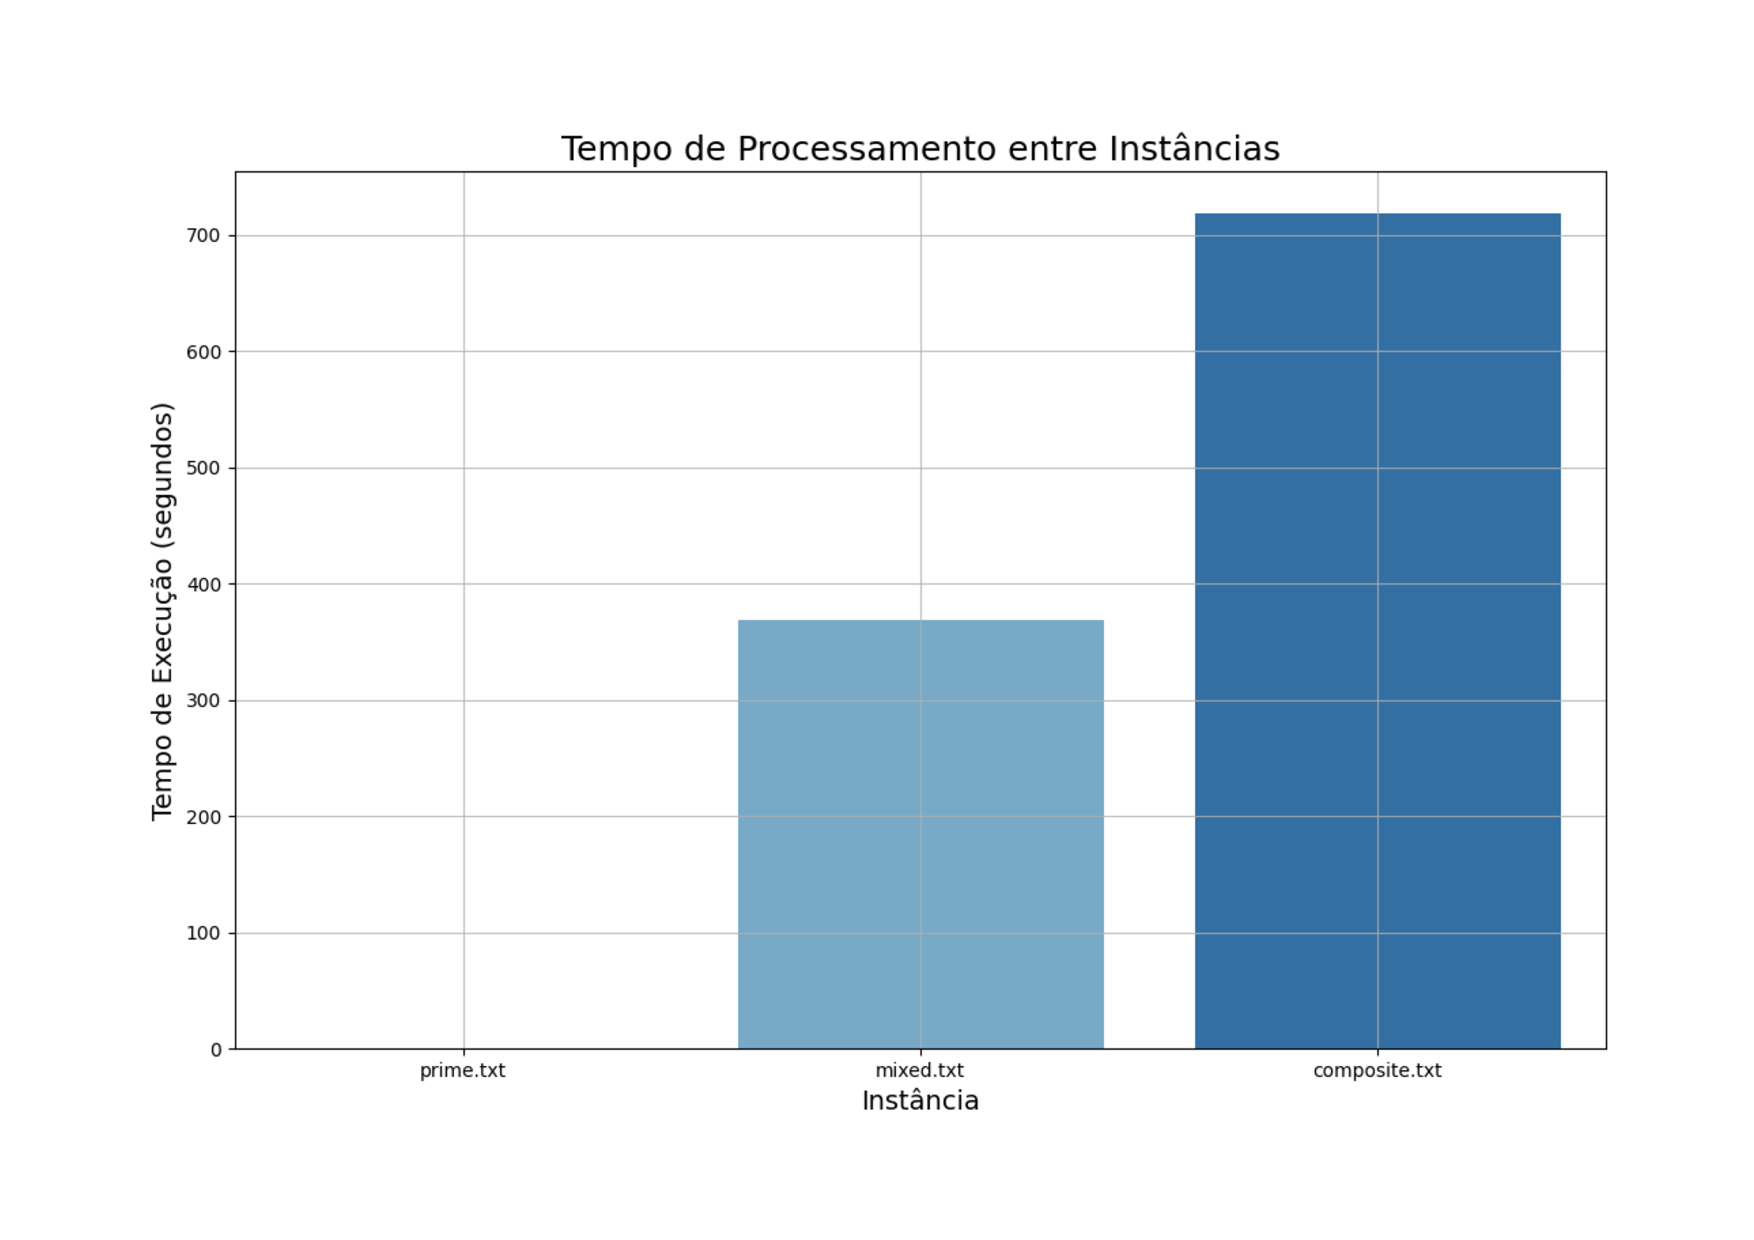
\includegraphics[width=1.1\textwidth]{Images/sequential.pdf}
    \vspace*{-1.5cm}
    \caption{Tempo de execução sequencial}
    \label{fig:map1}
\end{figure}

Como o tempo de execução para instâncias com 1000 valores contendo somente números primos é baixo, não há grandes variações na mensuração do mesmo variando o número de processos para execução em paralelo. Como mostra a Figura \ref{fig:map2}, embora ainda seja possível alcançar um \emph{speed up} de aproximadamente 2x em relação à execução sequencial, aumentar o número de processos poderá eventualmente provocar piora no tempo de execução devido ao aumento da comunicação entre processo mestre e escravos.

\begin{figure}[H]
    \centering
    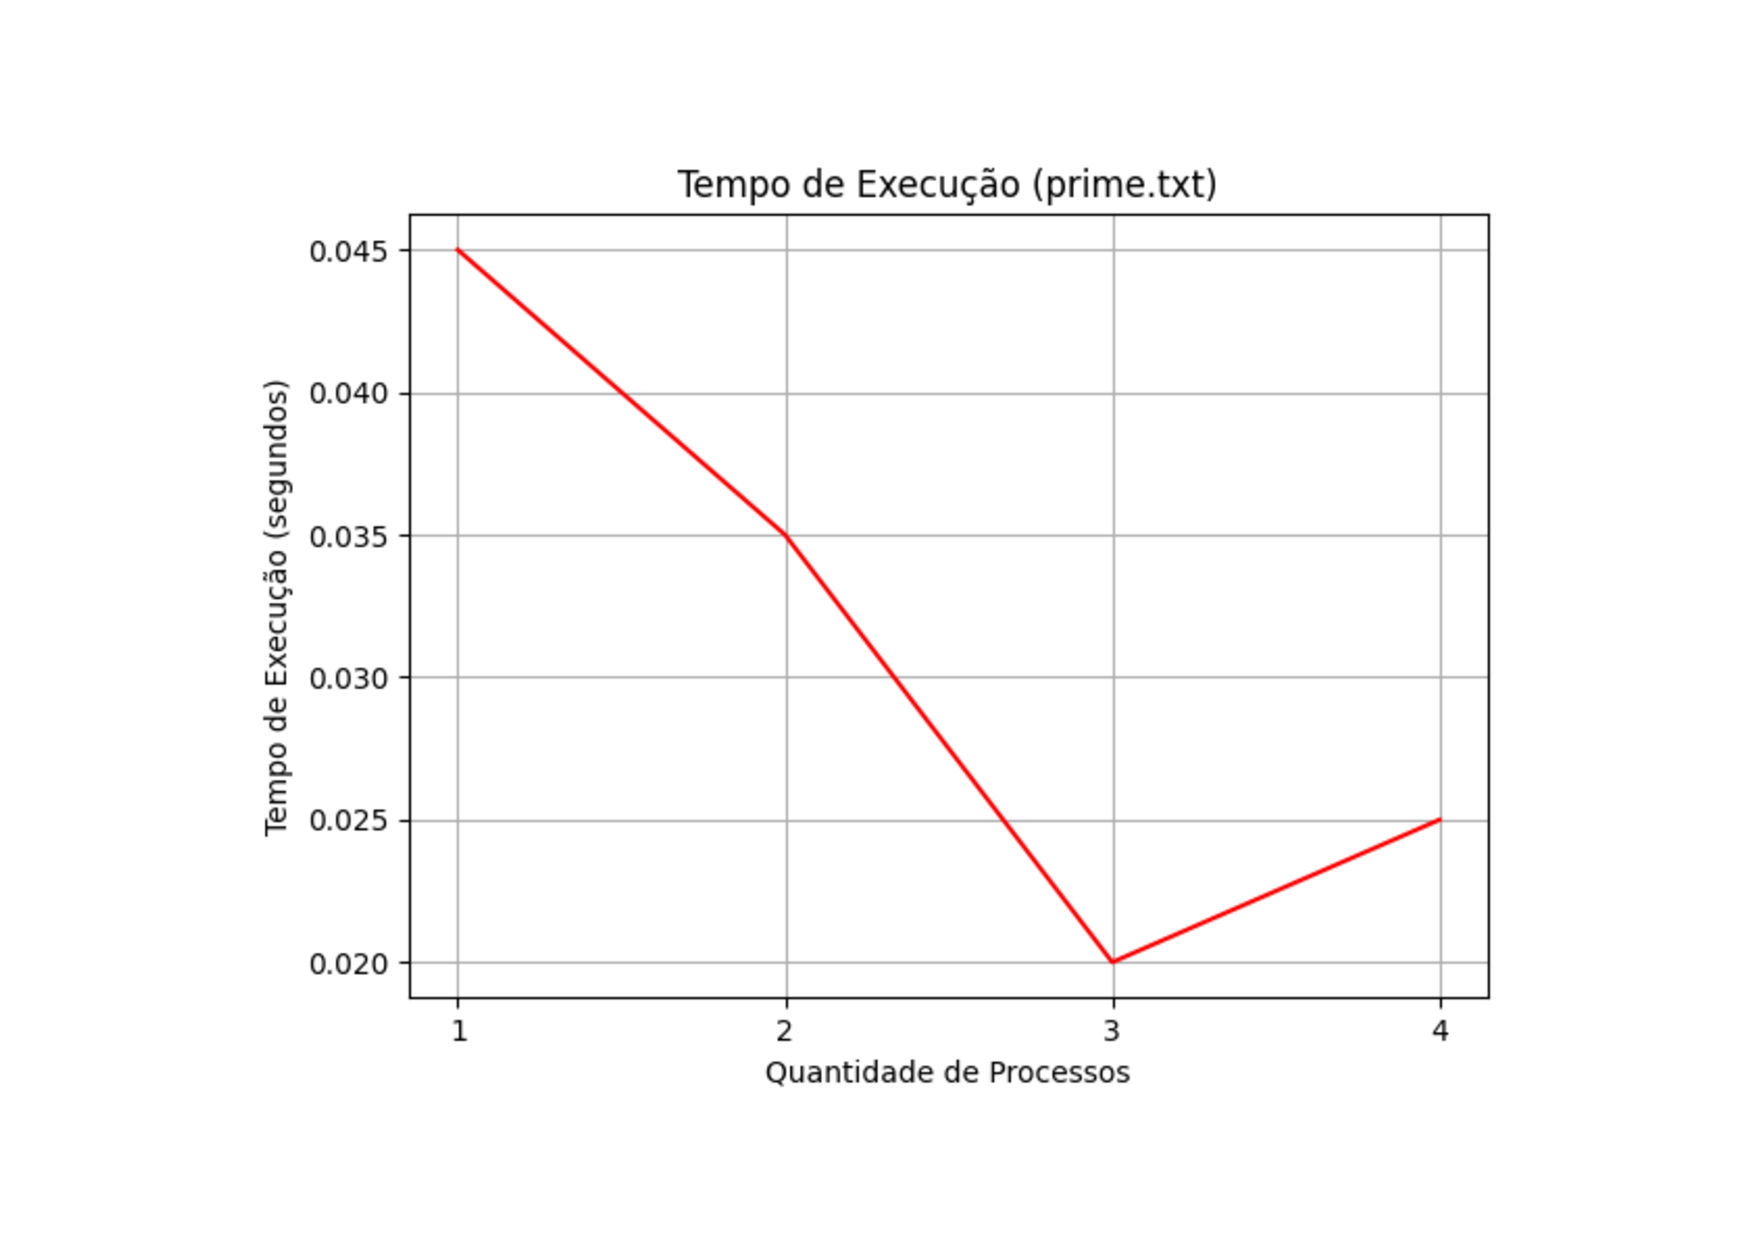
\includegraphics[width=1.1\textwidth]{Images/prime.pdf}
    \vspace*{-1.5cm}
    \caption{Tempos de execução com números primos}
    \label{fig:map2}
\end{figure}

Para execução das instâncias contendo somente números compostos e a mistura de ambos, o aumento no número de processos certamente promoveu ganhos no tempo de execução dos programas. Como mostrado na Figura \ref{fig:map3} e \ref{fig:map4}, o aumento gradual do número de processos provocou um \emph{speed up} de aproximadamente 2,4x e 2,6x em relação à execução sequencial para as instâncias composta e mista, respectivamente. No entanto, é nítido que os ganhos em tempo de execução não são inversamente proporcionais ao aumento do número de processos (e.g., 4 processos, tempo 4x menor). Tal observação pode ser explicada novamente pelo aumento na comunicação entre processos.

\begin{figure}[H]
    \centering
    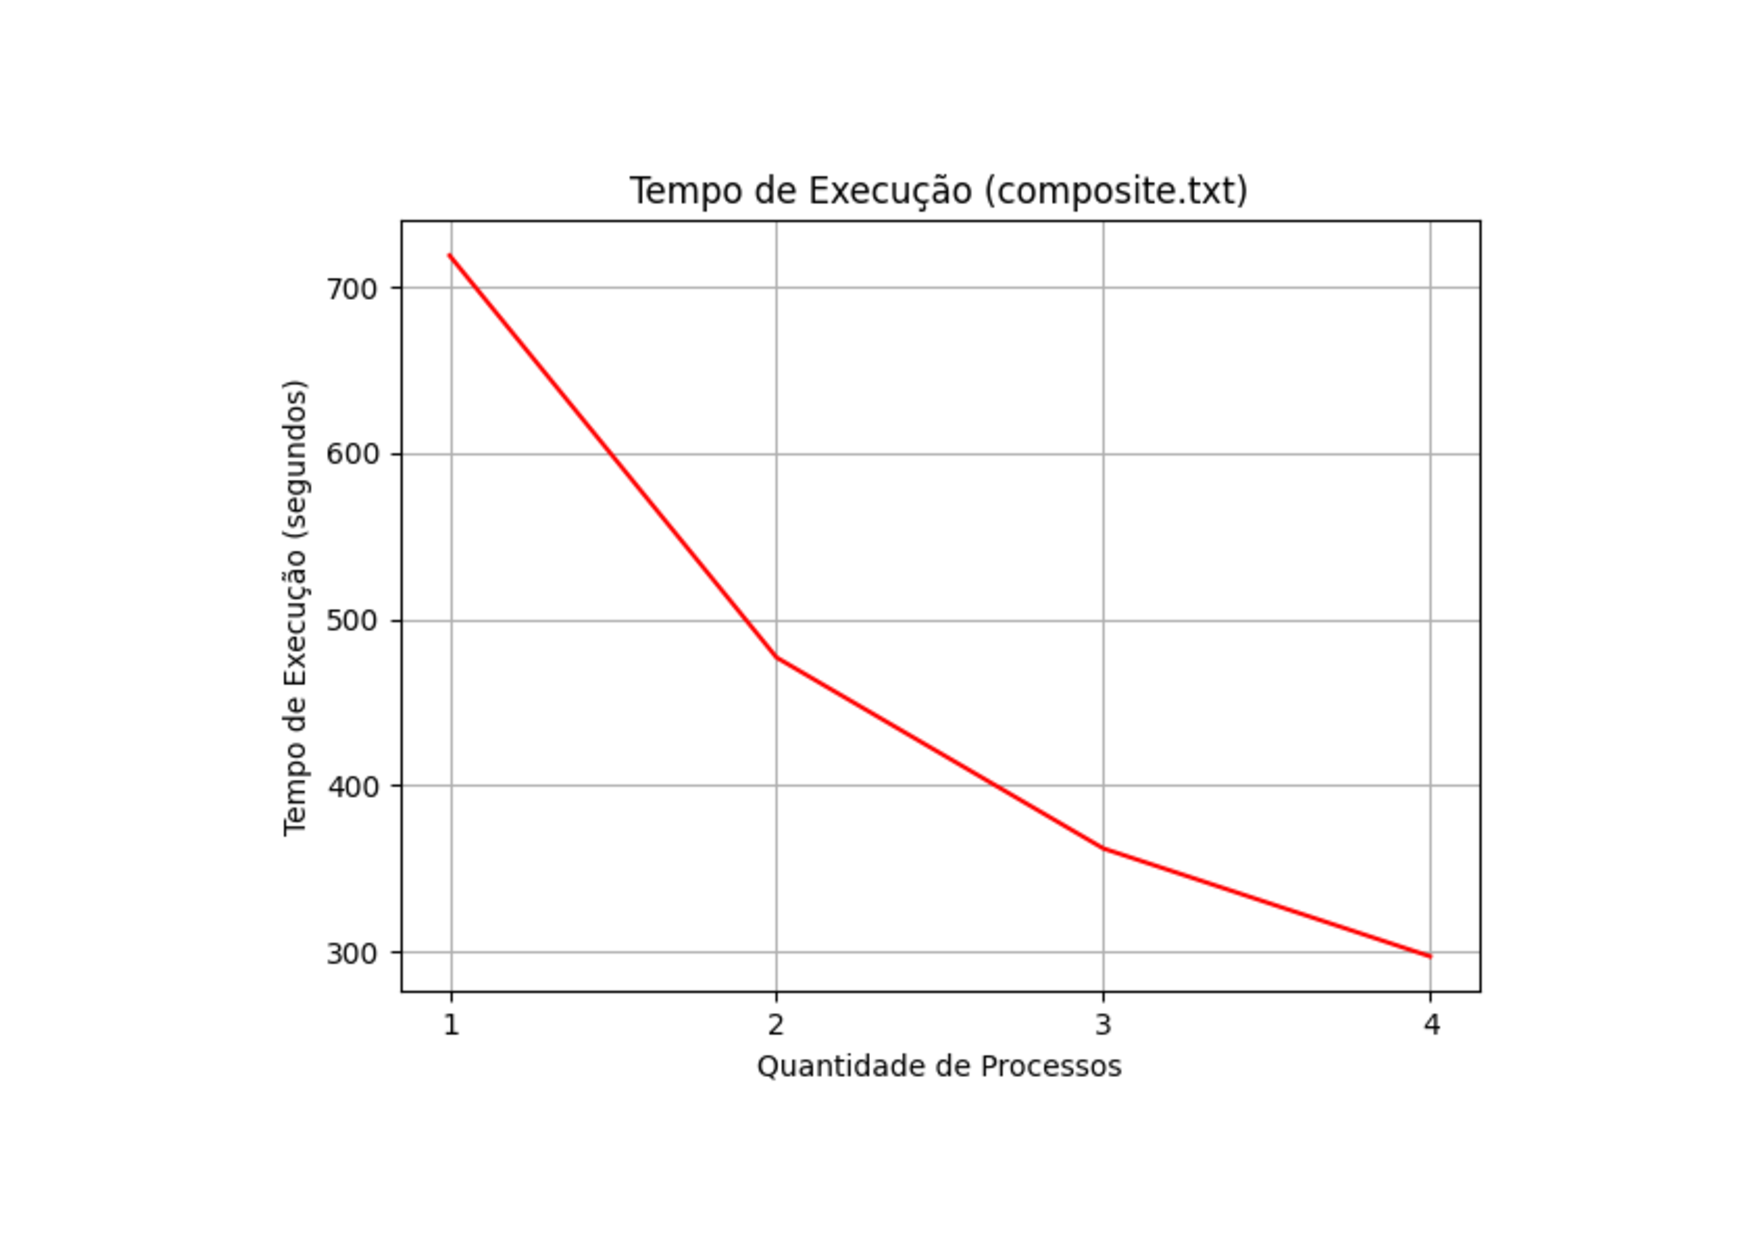
\includegraphics[width=1.1\textwidth]{Images/composite.pdf}
    \vspace*{-1.5cm}
    \caption{Tempos de execução com números compostos}
    \label{fig:map3}
\end{figure}

\vspace*{-1.8cm}
\begin{figure}[H]
    \centering
    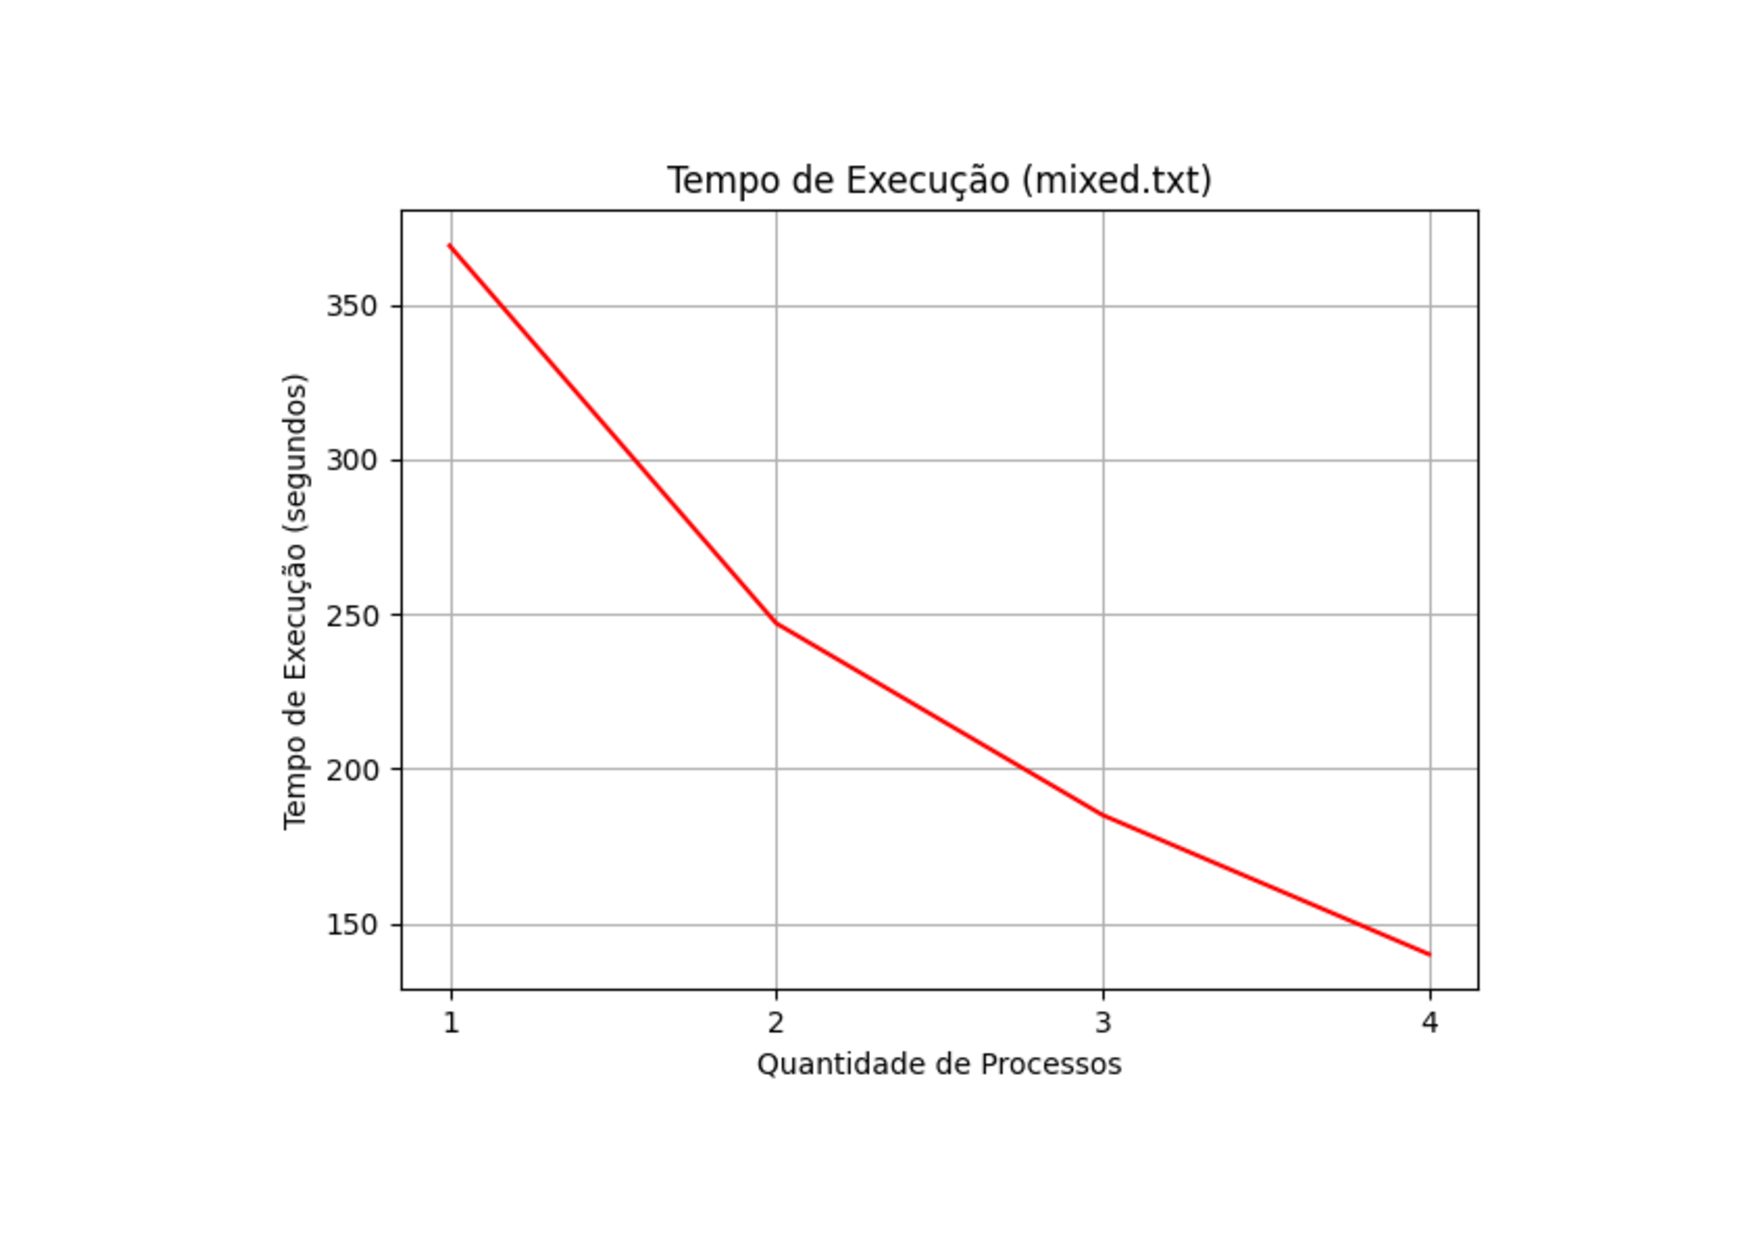
\includegraphics[width=1.1\textwidth]{Images/mixed.pdf}
    \vspace*{-1.5cm}
    \caption{Tempos de execução com números primos e compostos}
    \label{fig:map4}
\end{figure}

Por fim, podemos observar na Figura \ref{fig:map5} o quadro geral das execuções sequenciais e em paralelo, com diferentes números de processos e instâncias de tipos distintos. A paralelização do programa certamente trouxe ganhos em tempo de execução para execução com entradas mistas e compostas. No entanto, não é possível obter conclusões significativas sobre o ganho com entradas primas. Para mensurar a eficiência do programa com este tipo de entrada, é necessário gerar instâncias significativamente maiores para experimentação.

\vspace*{-1.3cm}
\begin{figure}[H]
    \centering
    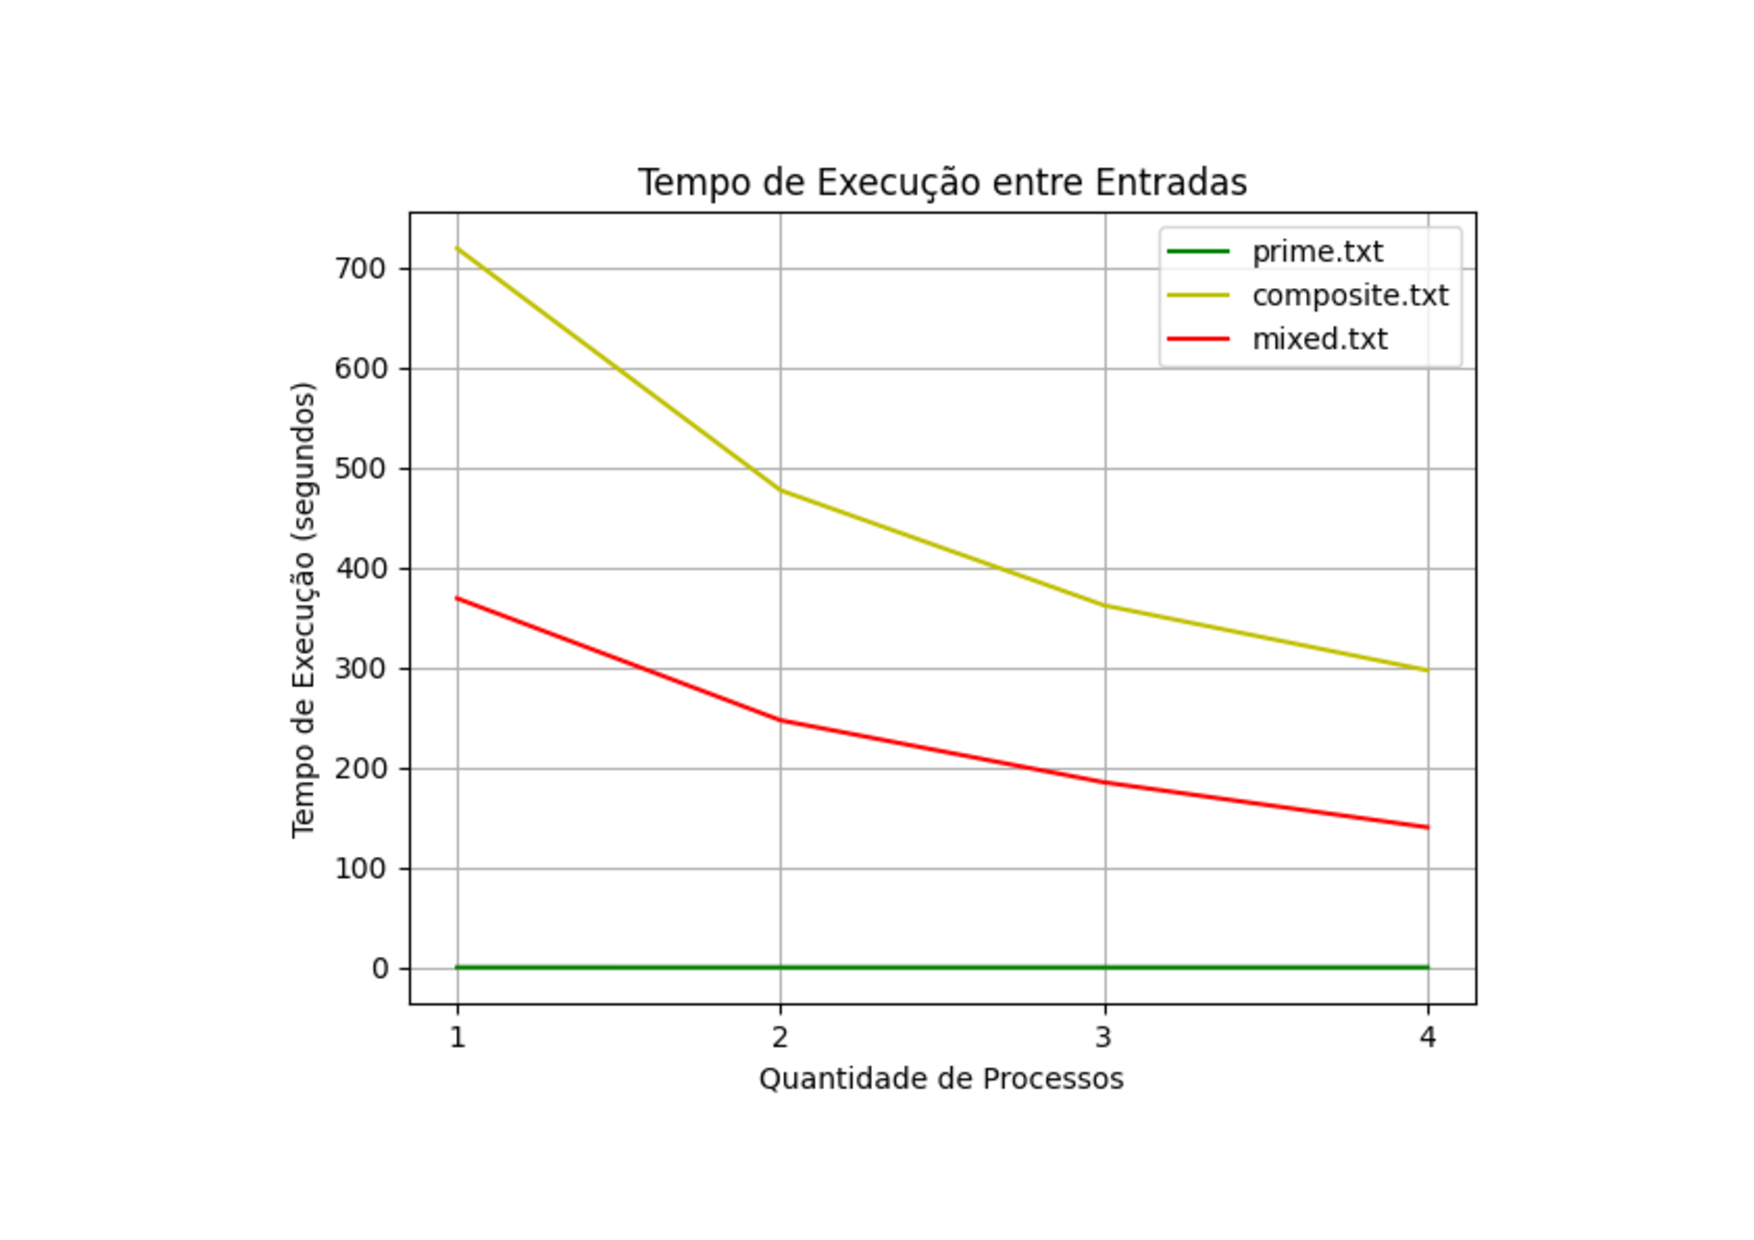
\includegraphics[width=1.1\textwidth]{Images/parallel.pdf}
    \vspace*{-1.5cm}
    \caption{Tempos de execução variando número de processos e entradas}
    \label{fig:map5}
\end{figure}

\section{Limitações}

Como principal limitação, é possível citar o descumprimento parcial do modelo mestre-escravo. Na utilização da rotina \emph{MPI\_Scatterv}, os fragmentos do arquivo de entrada são particionados de forma que todos os processos envolvidos no comunicador recebem um fragmento (Figura \ref{fig:map6}). Em outras palavras, o processo mestre que deveria apenas ser responsável pelas operações de E/S (carregando o arquivo de entrada para a memória e armazenando o resultado em um arquivo de saída), também realiza o processamento do número de divisores de uma porção dos dados de entrada.

\begin{figure}[H]
    \centering
    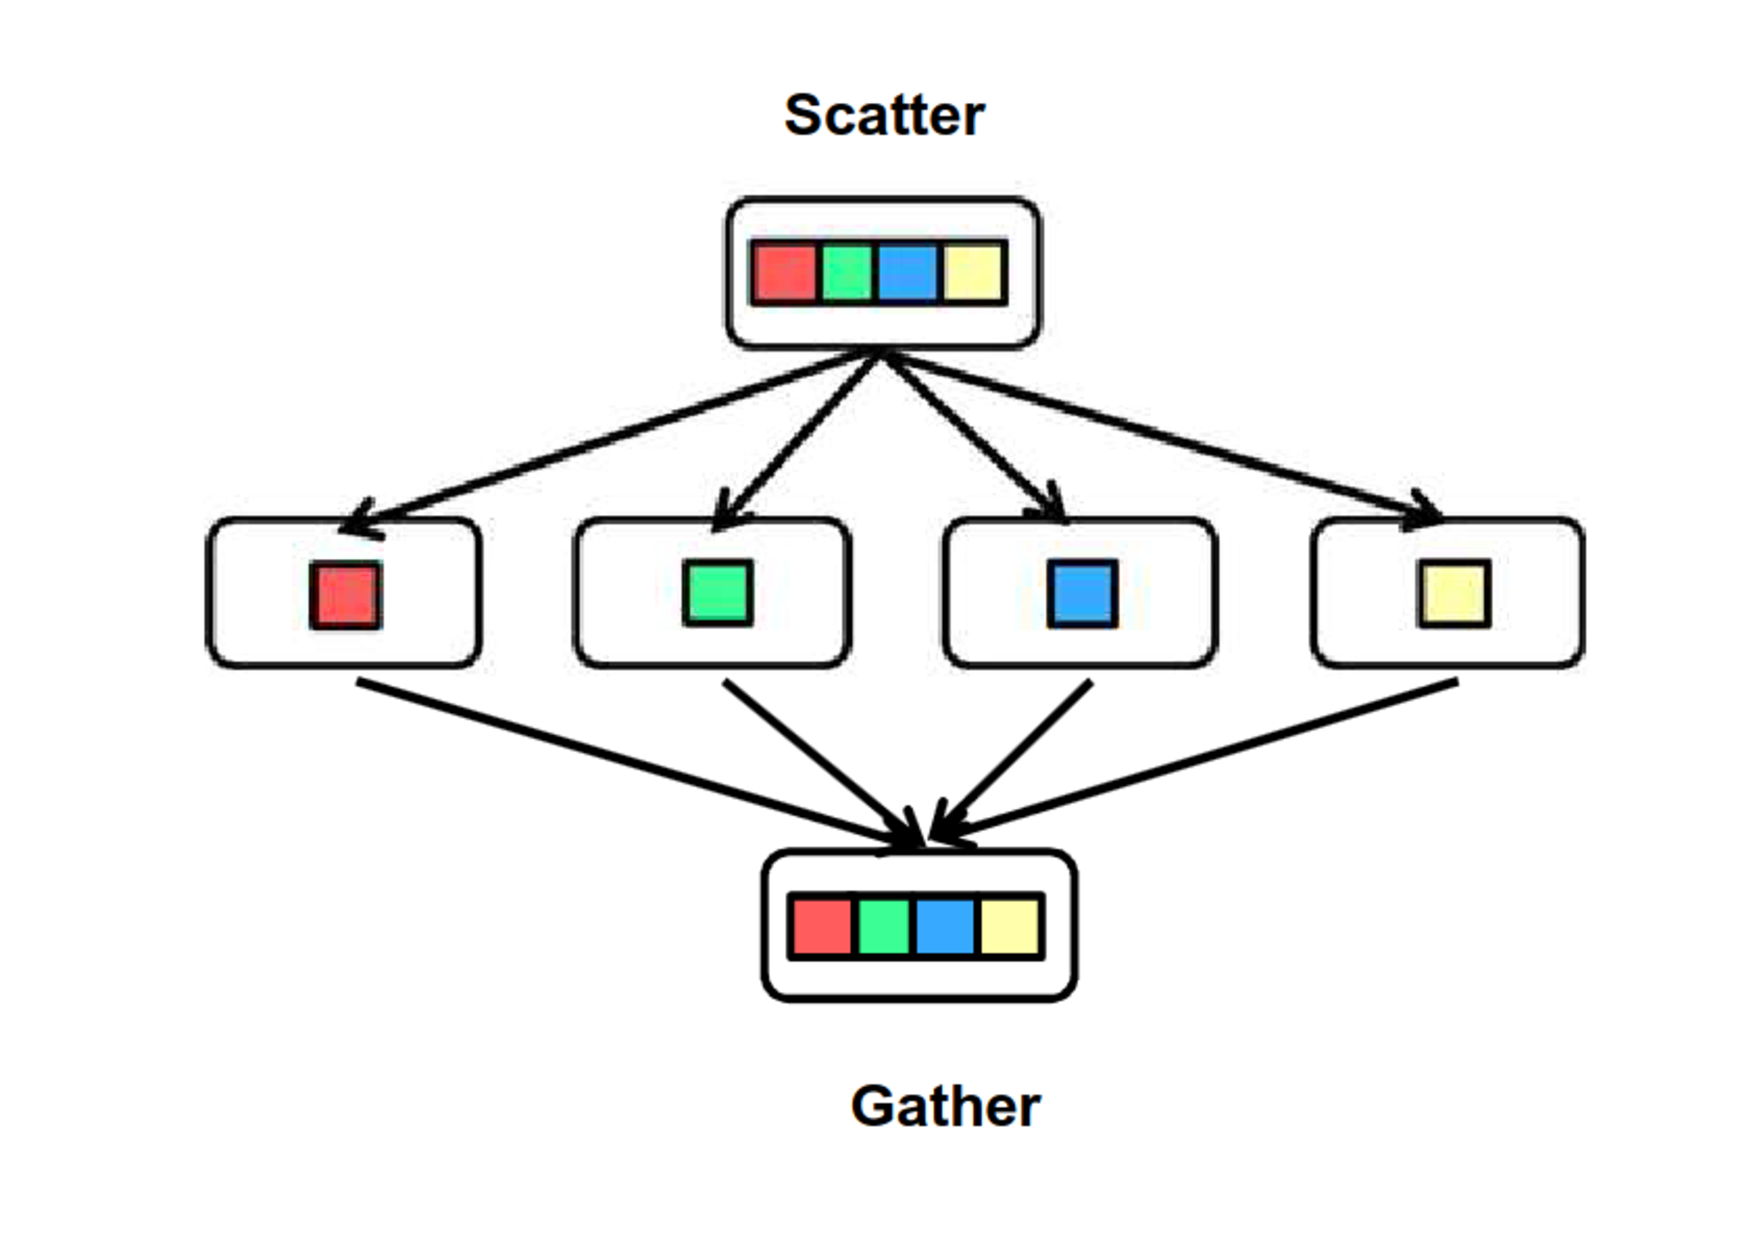
\includegraphics[width=0.85\textwidth]{Images/scatterv.pdf}
    \caption{Princípio de funcionamento das rotinas \emph{Scatter}}
    \vspace{0.2cm}
    \hspace*{15pt}\hbox{\small Fonte:\thinspace{\small \small{Mike Bailey, Oregon State University}\footnotemark}}\\
    \label{fig:map6}
\end{figure}

\footnotetext[7]{\scriptsize{Disponível em: \url{https://web.engr.oregonstate.edu/~mjb/cs575/Handouts/mpi.2pp.pdf}}}

Para contornar tal obstáculo, é possível criar um comunicador restrito aos processos escravos, para que então possa ser realizada a operação de \emph{Scatter} com o primeiro processo escravo como raiz (\(rank = 1\)), distribuindo os dados somente entre os processos escravos. Posteriormente o agrupamento dos dados seria realizado no comunicador global, para que então o processo mestre possa armazenar o resultado em um arquivo de saída.

Outro obstáculo encontrado no desenvolvimento deste trabalho foi a execução em ambientes distribuídos. Surgiram diversas adversidades quanto às tentativas de conexões via SSH\footnotemark \hspace{0.1cm}com as máquinas presentes nos laboratório do DComp. Por isto, não foi possível coletar resultados sobre o tempo de execução de processos em máquinas distintas, o possível atraso que a comunicação por rede poderia acarretar na execução do programa, a utilização dos recursos computacionais como memória principal, e o eventual \emph{speed up} que tal forma de execução poderia oferecer. 

\footnotetext[8]{\scriptsize{Mais informações disponíveis em: \url{https://www.openssh.com/manual.html}}}

\section{Conclusão}

Neste trabalho, foi explorada uma abordagem de computação paralela utilizando a biblioteca OpenMPI para um problema bastante simples, mas no qual foi possível explorar diversos conceitos como decomposição de domínio, granularidade e paradigmas como mestre-escravo e SMPD (Single Program Multiple Data).

Com este exemplo didático, podemos observar de forma nítida, a complexidade por trás de construir um programa que será executado em todos os processos (núcleos e/ou máquinas) de forma indiscriminada. Por isto, sempre é necessário ter extrema cautela no controle dos \emph{ranks} de cada processo, assim como a alocação e o acesso a memória realizado por cada um, principalmente em um ambiente de computação com memória distribuída.

\section*{Referências}

\begin{itemize}
    \item The Message Passing Interface (MPI) - Parallelism on Distributed CPUs: \url{https://web.engr.oregonstate.edu/~mjb/cs575/Handouts/mpi.2pp.pdf};
    \item Profiling Programs With prof, gprof, and tcov: \url{https://docs.oracle.com/cd/E19059-01/stud.10/819-0493/OtherTools.html};
    \item scatter variable length data: \url{https://stackoverflow.com/questions/43642561/scatter-variable-length-data};
    \item Executing Shell Commands from a C program: \url{https://www.cs.uleth.ca/~holzmann/C/system/shell_commands.html};
    \item Material disponível no SIGAA na disciplina de Computação Paralela.
\end{itemize}

\end{document}